\section{Experimental Results}
\label{sec:exp}

This section presents the results of our experiments on the finite-field multipliers.
We compare an implementation of \textcolor{red}{Algorithm (mention the algo. no.)}  
against  the incremental SAT based approach presented in \textcolor{red}{Fujita's paper reference}.
We have implemented the approach presented in \textcolor{red}{Fujita's paper reference} using
Python and PICOSAT as the underlying SAT solver. The experiments are performed on a 4.0GHz 
Intel(R) $\text{Core}^{\text{TM}}$ i7-6700K Quad-Core CPU with 32 GB of RAM.   

\subsection{Mastrovito Multipliers}
Modular multiplication is an important operation used in cryptography. 
A Mastrovito multiplier architecture can be used for performing this computation.
Mastrovito multipliers compute $Z = A\times B \pmod{
  P(x)}$ where $P(x)$ is a given primitive polynomial for the datapath size
$k$. 

The product $A \times B$ is computed using an array multiplier architecture, and then the result is reduced modulo $P(x)$.
The following example demonstrates the Mastrovito multiplier computation~\cite{lv:tcad2013}.
%take $\{A,B\} =
%\{a_0,a_1,\dots,a_{k-1},b_0,b_1,\dots,b_{k-1}\}$ as $k$-bit inputs and
%produce $Z = \{z_0,z_1,\dots,z_{k-1}\}$ as $k$-bit output. The multiplier
%performs $Z = A \times B \pmod{P}$, 

%The procedure 
%involves computing the product $S=A\times B$ using an array multiplier
%and then reducing it $\pmod{P}$ to obtain $Z$. We perform experiments
%on \textit{flattened} netlists of these circuits.  

\begin{Example}
\label{exp1}
{\it 
Consider the field $\mathbb{F}_{2^4}$. Let the inputs be:
$A=a_0+a_1\cdot \alpha+a_2\cdot \alpha^2+a_3\cdot \alpha^3$ and
$B=b_0+b_1\cdot \alpha+b_2\cdot \alpha^2+b_3\cdot \alpha^3$, and 
 the irreducible polynomial be $P(x)=x^4+x^3+1$. 
 % We have to perform the multiplication $Z =A\times B \pmod{ P(x) }$. 
 The coefficients of $A = \{a_0, \dots, a_3\}, B = \{b_0, \dots, b_3\}$ are in
$\mathbb{F}_2 = \{0, 1\}$. First, we perform the multiplication as:

%\vspace{-0.2in}

\vspace{0.05in}

{\small
{\begin{tabular}{c c c c c c c c}
%\vspace{-0.2in}
  &   &   & $a_3$ & $a_2$ & $a_1$ & $a_0$  \\ 
 $\times$&   &   & $b_3$ & $b_2$ & $b_1$ & $b_0$  \\ 
 \hline
 &   &   & $a_3\cdot b_0$ & $a_2 \cdot b_0$ & $a_1\cdot b_0$ & $a_0\cdot b_0$ \\
 &  & $a_3\cdot b_1$ & $a_2\cdot b_1$ & $a_1 \cdot b_1$ & $a_0\cdot b_1$ &   \\
 & $a_3\cdot b_2$ & $a_2\cdot b_2$ & $a_1\cdot b_2$ & $a_0\cdot b_2$ &  &   \\
 $a_3\cdot b_3$ & $a_2\cdot b_3$ & $a_1\cdot b_3$ & $a_0\cdot b_3$ &  &  &   \\
 \hline
 $s_6$& $s_5$  & $s_4$  & $s_3$ & $s_2$  & $s_1$   & $s_0$ 
% \vspace{-0.2in}
\end{tabular}}
}

\vspace{0.05in}

The result $Sum = s_0+s_1\cdot \alpha + s_2\cdot \alpha^2 + s_3\cdot
\alpha^3 + s_4\cdot \alpha^4 + s_5\cdot \alpha^5 + s_6\cdot \alpha^6$,
where, $s_0  =  a_0\cdot b_0, ~~s_1  =  a_0\cdot b_1 + a_1\cdot b_0,
~~s_2 = a_0\cdot b_2 + a_1\cdot b_1 + a_2\cdot b_0$, and so on. Here
the multiply ``$\cdot$'' and add ``$+$'' operations are performed
modulo 2, and hence implemented in a circuit using AND and XOR
gates. As the coefficients are always reduced modulo $p =
2$, there are no carry-chains
in the design. Next, the result is reduced modulo the primitive
polynomial $P(x) = x^4 + x^3 + 1$, as:
% where the final output of the circuit is denoted by $G(x)  = g_3x^3
% + g_2x^2 +g_1x + g_0$.  

\vspace{0.05in}

{\small
{\begin{tabular}{|c c c c | l }
  $s_3$   &$s_2$    &$s_1$   &$s_0$   &   \\
 \hline
 $s_4$    &$0$    &$0$   &$s_4$   &$s_4\cdot \alpha^4 \pmod{P(\alpha)} = s_4 \cdot (\alpha^3 + 1)$\\
 $s_5$    &$0$    &$s_5$   &$s_5$     &$s_5\cdot \alpha^5 \pmod{P(\alpha)} = s_5\cdot (\alpha^3+ \alpha + 1)$\\
 $s_6$    &$s_6$    &$s_6$   &$s_6$     &$s_6\cdot \alpha^6 \pmod{ P(\alpha)} = s_6\cdot( \alpha^3 + \alpha^2 + \alpha + 1)$\\
 \hline
 $z_3$    &$z_2$    &$z_1$   &$z_0$   &
 \end{tabular}\par}
}

\vspace{0.05in}

The final output of the circuit is: $Z = z_0 + z_1 \alpha + z_2
\alpha^2 + z_3 \alpha^3$; where  $z_0=s_0+s_4+s_5+s_6; ~~z_1=s_1+s_5+s_6;
~~z_2=s_2+s_6; ~~z_3=s_3+s_4+s_5+s_6$. 
}
\end{Example}

\subsection{Montgomery Multipliers}
Exponentiation (repeated multiplication) is often required in cryptosystems.  
For such applications, Montgomery architecture \cite{acar:1998} \cite{wu:2002}
% \cite{Barrett:1987} 
\cite{Knezevic:2008} are considered more efficient than Mastrovito multipliers
as they do not require explicit reduction modulo $P(x)$ after each step.

Fig.~\ref{montfig} shows the structure of a Montgomery
multiplier. Each MR block computes $A\cdot B\cdot R^{-1}$, where $R$
is selected as a power of a base ($\alpha^{k}$) and $R^{-1}$ is the multiplicative 
inverse of $R$ in $\mathbb{F}_{2^k}$. As this operation cannot compute $A\cdot B$
directly, we need to pre-compute $A\cdot R$ and $B\cdot R$ as shown in the Fig.~\ref{montfig}. 
We denote the leftmost
two blocks as Block A (upper) and B (lower), the middle block as Block
C and the output block as Block D.
% We have presented results for GBR
%on both \textit{flattened} and \textit{hierarchical} netlists of these
% multipliers. 

\begin{figure}[H]
  \centering
  %\def\svgwidth{340pt}
  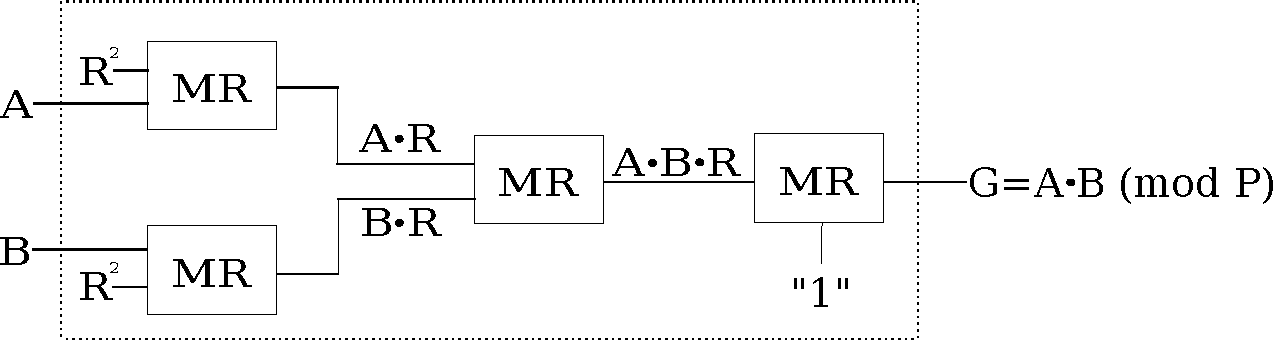
\includegraphics[scale=0.34]{new_mmcircuit-eps-converted-to}
  \caption{Montgomery multiplication.}
  \label{montfig}
  \end{figure}
\vspace{-0.1in}

Table \ref{masusmontspec} presents the execution times when there is an unknown component in the
Mastrovito multiplier  and Montgomery multiplier is used as the specification. The labels $no$, $md$, and $ni$ 
denote that the unknown component is near output, near input and somewhere in the middle, respectively.

\begin{table}[H]
\centering
\caption{\textcolor{red}{Some caption like: Unknown Component in Mastrovito mulitplier and Montgomery multiplier used as spec ....}( Time is in
seconds); k = Datapath Size of two multipliers, \#Gates = No. of gates, Time-Out = 12 hrs, K = $10^3$, M = $10^6$}
\label{masusmontspec}
\begin{tabular}{| c | c | c | c |} \hline
%\multirow{2}{*}{\textbf{Input}} & \multirow{2}{*}{\textbf{Abstraction}} & \multicolumn{3}{ c |}{\textbf{ZBDD reduction(ZR)}}  &  \multirow{2}{*}{\textbf{ZR improved}}\\ \cline{3-5}
% & &Building ZBDDs&Reduction&Total&\\ \hline
\multirow{2}{*}{\textbf{k}}& \multicolumn{3}{ c |}{\textbf{\textcolor{red}{Fujita's paper reference}}}\\ \cline{2-4}
&{\it no}&{\it md}&{\it ni} \\ \hline
9&33.7&36.8&34.9 \\ \hline
10&214.3&215&231.4 \\ \hline
11&1,999.5&1,927&2,090.7 \\ \hline
12&24,085&23,400& (still running) \\ \hline
13&TO&TO&running (will TO) \\ \hline
\end{tabular}
\end{table}